\chapter[De l'individu à la population: quand la densité dépendense casse la
règle taille~--~température][Densité dépendance et température]{De l'individu à la population: quand la densité dépendance casse la
règle taille~--~température}
\label{Ann:fip}

\vspace{2cm}

\texttt{
Mallard, François, Vincent Le Bourlot, Christie Lecoeur, and Thomas Tully, ``From
individuals to populations:
density dependence effects break the temperature-size rule''\\
under review at Journal of Animal Ecology
}

\section*{Abstract}
\addcontentsline{toc}{section}{Summary}

\lettrine[lines=3]{D}{ensity-dependence} complicates the task of predicting the
effect of climate change on populations. Life history traits are known to be plastic in response
to temperature: adult size of most ectotherms follows the so-called
temperature-size rule. Life history traits are also known to be density
dependent. In turn, density-dependence may be modulated by temperature. Here we
aim at disentangling the effects of temperature, density dependence and the
interaction between temperature and density effects, by comparing reaction norms
of isolated individuals to the observed traits of individuals in dynamic
populations, across a wide range of temperatures. Using the Collembola Folsomia
candida, we describe the reaction norms of maturation length, growth rate and
asymptotic size over a large temperature range (6 to 26$\degres$C) and examine
the structure and dynamics of populations reared under the same temperatures for
three years. We use reaction norms to predict variation of adult size and growth
rates measured in the populations. We found that the population dynamics and
population size structure depend on temperature but that the individual-level
reaction norms are overruled by density dependent effects. For a given
temperature, competition can result in individuals that reach a larger body
length, which leads to a reduced population density. We argue that high
temperature speeds up the life cycle and induces a change of the perceived food
provisioning in the populations that alters the competition for resources. This
underlines the need to untangle the complex interactions between environment and
demography to help predicting how climate change influences population dynamics.

\section{Introduction}

Long term studies of natural populations have shown that environmental changes
can lead to shifts in life history trait
distributions\autocites{parmesan2006a,ozgul2009a}. These shifts can be difficult
to predict because of interactions between ecological and evolutionary processes
\autocites{kokko2007a}. The ambient temperature is well known to influence life
history traits \autocites{atkinson1996a,angilletta2009a}, such as age or size at maturity, as represented by the temperature-size rule
\autocites{berrigan1994a,fischer2002a,dhillon2004a}. How predictable the
alterations of these traits are in the wild, owing to temperature change, is
still widely debated \autocites{gardner2011a,sheridan2011a}.
To study the influence of temperature change on phenotypes, a classical approach
is to measure reaction norms \autocites{woltereck1909a}, usually on isolated
individuals \autocites{driessen2007a,ellers2011a} or small cohorts
\autocites{karan1998a,liefting2009a} raised over a range of temperatures.
Although these laboratory experiments can tell us a lot about how environmental
conditions alter individual phenotypes, their applicability to the way a
population responds is limited since temperature affects not only the
physiology of each individual but also the size and structure of populations
which themselves affect the traits of individuals through density dependent
feedback regulations.

A temperature change may induce plastic modifications in resource allocation
towards growth, reproduction or maintenance efforts. In populations, a variation
of ambient temperature may also affect competition between individuals of
different sizes by affecting not only their consumption and metabolism rates,
but also by changing the renewal rate of resources.

Our aim here is to investigate how thermal reaction norms measured on isolated
individuals can help in understanding and predicting population structure and
dynamics over a large temperature range. More specifically, we measured how the
direct effects of temperature on the life history of individuals are modulated
by the indirect demographic feedback loop (Figure \ref{Fig5-1}). To do so, we followed
isolated Collembolans (Figure \ref{Fig5-2}a). Figure \ref{Fig5-3} shows the thermal reaction norms (11 to
26$\degres$C) of maturation size, growth rates and asymptotic size. This provides a
reference measure for the direct effects of temperature on the phenotype of
individuals (arrow 1, Figure \ref{Fig5-1}). We then examined the size-structure and density
of populations bred under the same range of temperatures (Figure \ref{Fig5-2}d) and monitored
weekly over almost three years, representing many generations and providing
details on cohort growth rates and asymptotic body lengths. We finally combined
these two experiments and used the reaction norm measurements to estimate the
deviation of the individual phenotypes due to the density dependence (arrow 4,
Figure \ref{Fig5-1}) in order to discuss the effect of temperature (arrow 2, Figure \ref{Fig5-1}).

\begin{figure}[!ht] % Figure 1 
\centering
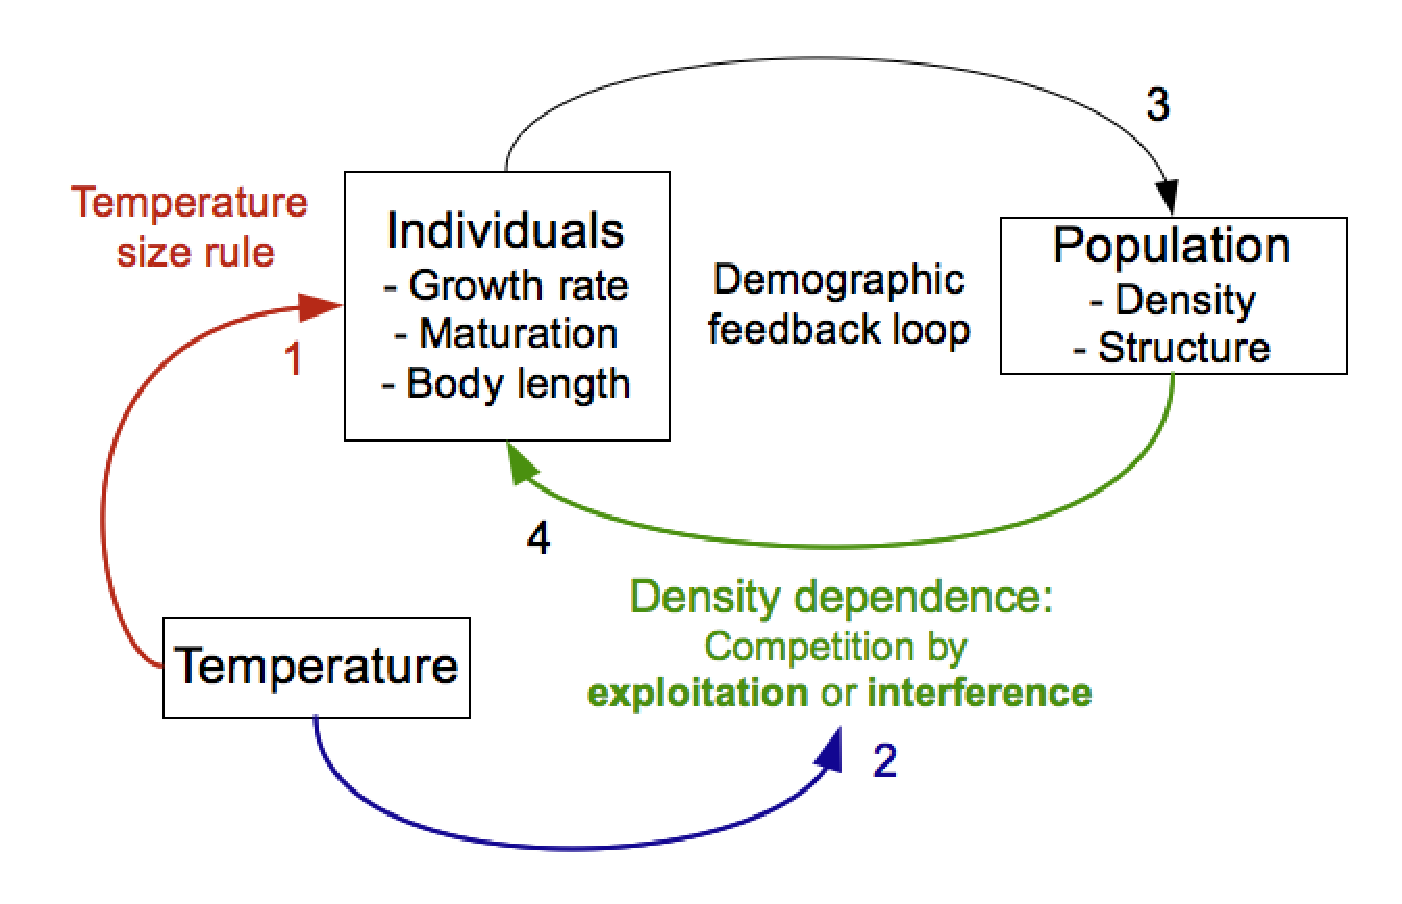
\includegraphics[width=0.85\textwidth]{5_ChapExp3/fig/Fig1}
\caption[\lofimage{5_ChapExp3/fig/Fig1}Direct and indirect
effects of temperature]{Schematic representation of the direct (1) and indirect
(2+4) effects of temperature on the life history traits of individuals.}
\label{Fig5-1}
\end{figure}

\section{Material and methods}

\subsection{Model organism}

The model organism used in this study, the Collembola Folsomia candida, is a
small ($\approx2$mm long)  blind ametabolous hexapod (Figure \ref{Fig5-2}a) broadly distributed
throughout the world. They are found in habitats such as decaying litter,
rotting wood or in caves \autocites{fountain2005a}. It is easy to
breed and maintain individuals or populations in the laboratory in very simplified
microcosms (Figure \ref{Fig5-2}d) whose main parameters can be finely controlled
(temperature, food, density, humidity). Every stage of a life-cycle is visible
(eggs, nymphs, adults) and measurements and environmental manipulations can be
done on both nymphs and adults since they share the same environment, eat the
same food and have the same ecology. They grow by moulting about twice a week at
21$\degres$C during their whole life time. This species is known to demonstrate
highly flexible phenotypic adjustments when experiencing a sudden change in density or
resource abundance \autocites{tully2008a}. As a parthenogenetic
species, multiple individuals sharing the same genotype can easily be bred in different
environmental conditions. We worked with two distinct genetic clonal lineages
(labelled respectively TO and HA) with contrasted ecological history and
bio-demographic strategies \autocites{tully2006a,tully2008a}.

\begin{figure}[!ht] % Figure 2 
\centering
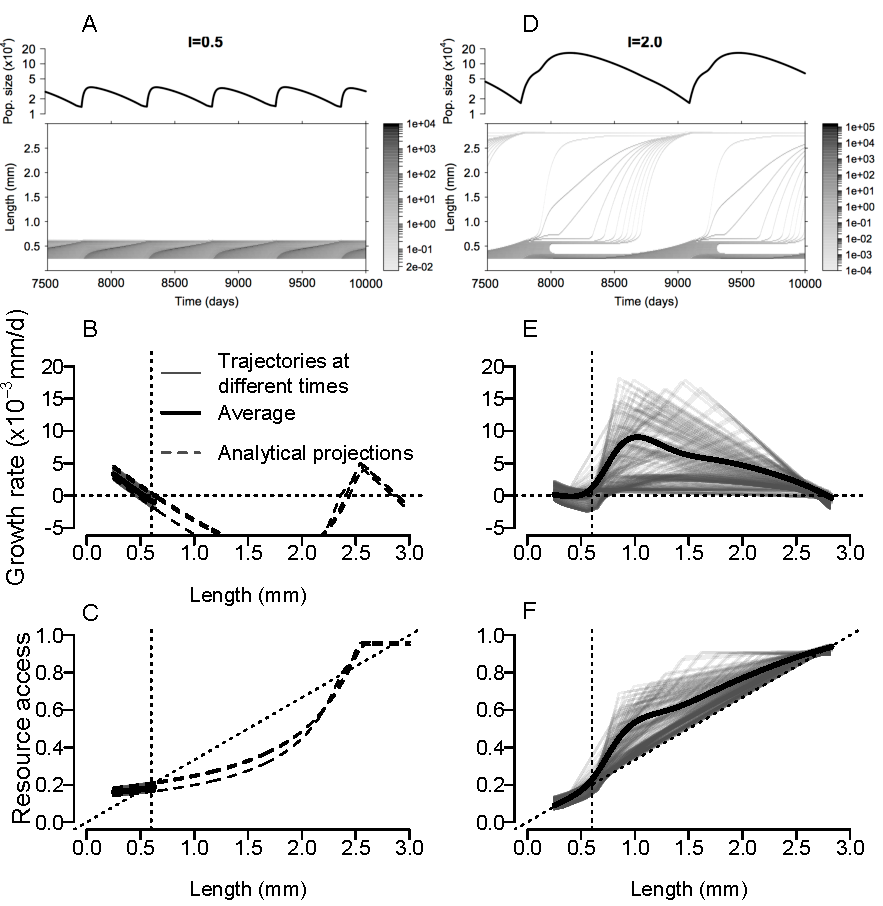
\includegraphics[width=0.95\textwidth]{5_ChapExp3/fig/Fig2}
\caption[\lofimage{5_ChapExp3/fig/Fig2}Measurements of the juvenile growth rate and mean adult body length]{
Measurements of the juvenile growth rates and mean adult body lengths have been
made on isolated individuals (a) and in the populations (b). The growth
trajectories of two individuals (b, c) and the size-structure dynamics of two
populations (e, f) raised under two different temperatures (b, e:11$\degres$C; c, f:
26$\degres$C) are presented as examples. On isolated individuals (b, c), a logistic
growth curve (red) was fitted to the measurements (black dots) to estimate the
growth rate at the inflexion point (blue lines) and the asymptotic body length.
In the populations (e, f), growth rates were measured as the slope of mean body
length with time for distinguishable cohorts (black lines) and mean adult length
was estimated when the mean size of the cohorts had stabilised (points)}
\label{Fig5-2}
\end{figure}

\subsection{Rearing conditions}

Both isolated individuals (Figure \ref{Fig5-2}a) and populations (Figure \ref{Fig5-2}d) were kept in
standard rearing boxes made of polyethylene vials (diameter 52 mm, height 65 mm)
filled with a 30 mm layer of plaster of Paris mixed with 600 mL of Pébéo
graphic\copyright~Chinese ink to increase visual detectability of individuals
against the background \autocites{tully2008a}. Food was provided once a week
in the form of small pellets of a mixture of dried yeast and agar in standardised concentration
and volume (5000 mL water+80 mg agar+800 mg dried yeast, to produce pellets of
15 $\mu$L). Both isolated individuals and populations were kept in incubators
(FOC 225E, temperature controlled $\pm$0.5$\degres$C), at constant humidity
($\approx$ 100\%) and in darkness.

\subsection{Thermal reaction norms of isolated individuals}

Newborn individuals were isolated immediately after hatching and fed ad libitum
during their whole life. We randomly placed individuals of each clone at each
temperature within our range (11, 16, 21, 26 and 29$\degres$C, Table \ref{tab5-1}). The
body lengths of the individuals were measured at the beginning of the experiment,
then three times a week during ten weeks and then once a week. For each body
length measurement two to three pictures were taken using a digital camera
(Nikon D300) fixed on a dissecting scope. Body length was measured on each
picture using the ImageJ software (\citealp{abramoff2004a},
\url{http://rsbweb.nih.gov/ij/}). The containers were regularly inspected for
eggs to assess age at maturation. Logistic growth curves were fitted to each individual
growth trajectory (Figure \ref{Fig5-S1}). Average maximal growth rates and
asymptotic sizes were estimated using non-linear least squares models fitted separately for each
individual growth trajectory (Figure \ref{Fig5-2}b, c) using the methods
described by Pinheiro \autocites{pinheiro2000a}. Linear models were
used to test for fixed effects (clonal identity and temperature being used as categorical
variables) on these two parameters.

\begin{table}[!ht]
\centering
\caption{
Number of isolated individuals followed since birth and populations followed
during more than one year of the two clones and for the four temperatures. The
number of individuals whose asymptotic length has been observed is in
brackets.}\label{tab5-1}
\begin{tabular}{ccccc}
\hline
\multirow{2}{*}{temperature} 
	& \multicolumn{2}{c}{Number of isolated individuals}
	& \multicolumn{2}{c}{Number of populations}\\
%case vide
	& HA
	& TO
	& HA
	& TO\\
\hline
11$\degres$C 
	& 4 (5)	
	& 5 (4)	
	& 4	
	& 4\\
16$\degres$C
	& 6 (5)	
	& 9 (8)	
	& 4	
	& 4\\
21$\degres$C
	& 7 (4)	
	& 6 (2)	
	& 12 
	& 12 \\
26$\degres$C
	& 6 (5)	
	& 9 (7)	
	& 4	
	& 4 \\
\hline
\end{tabular}
\end{table}

\subsection{Population dynamics and cohort growth rates measurements}

Populations were set up with five adults and maintained at the same temperatures
as the isolated individuals (11, 16, 21 and 26$\degres$C). To avoid any transient
effect, we only analysed the dynamics of these populations after being
maintained during at least one year at these temperatures. Four populations of
both clones were started at each temperature, and an extra eight populations
were added at 21$\degres$C (Table \ref{tab5-1}).

The population size structure was measured weekly during more than a year using
a dedicated plugin \autocites{mallard2012a,mallard2013a} of the ImageJ software
(\citealp{abramoff2004a}, \url{http://rsbweb.nih.gov/ij/}). Each
measurement gives us the number of individuals and for each individual counted, its length and its surface (which we refer to
as its biosurface). We extracted the life history traits (adult body length and
juvenile growth rate) in populations using the graphical representation for
structured time series (Figure \ref{Fig5-2}e, f, Figure \ref{Fig5-S2}) provided by the R
package STdiag (se  Chapter \ref{Chap:STDiag}).

\subsection{Thermal reaction norms of demographic traits}

We measured juvenile growth and adult body length by hand on the population
dynamics structured-time diagrams, using cohorts growing within the group of
adults (Figure \ref{Fig5-2} and Figure \ref{Fig5-S2}). Growth rate of each
cohort was measured by taking the slope of the mean body length in the cohort
against time. Finally, the asymptotic adult body length of each cohort was taken
as the average length of the adults once the growing cohort fully merged with
the preexisting adults, or when the average length of the growing cohort
stabilises (Figure \ref{Fig5-2} and Figure \ref{Fig5-S2}). We extracted the
number of individuals and the size of each individual during the periods when
corresponding to the measurements of growth rate or adult body length. This
count was used to measure the density of adults at the time of each measurement.
Individuals are considered adults if their length is greater than 0.8mm.

\subsection{Measuring the thermal reaction norms for growth rate and adult size
in populations}

In populations the growth rate and asymptotic adult body length are determined
by direct effects of temperature, direct effects of population (density) and
also potential interactions between temperature and density (Figure \ref{Fig5-1}). To
specifically focus on the latter two effects while controlling for the direct
effects of temperature (thermal reaction norms on isolated individuals), we did
not analyse directly the growth rates and adult lengths in populations but we
used two indexes that compare the traits measured in populations with the
measurements made on isolated individuals.

For the growth rates, we created a linear model explaining the ratio between the
observed growth rates in the populations and the average maximal growth rate of
isolated individuals at the same temperature. The adult density (number of
adults in the container), the temperature (used as a continuous variable here),
the clone identity and their interactions were used as explanatory variables.

Similarly, to take into account the variation of adult body length and size at
maturity of isolated individuals with temperature, we made up, for each
measurement of adult length in the populations, an index called the ``Growth
effort beyond maturation'' (GEBM). This GEBM is the proportion of the length that
adults grow to in addition to the maturation length and in relation to the
asymptotic length observed in isolated individuals. At each temperature, the
maturation and the asymptotic body lengths measured on isolated individuals, are
used as references to scale the asymptotic adult body lengths observed in the
populations. At a given temperature, this ratio indicates how much individuals
invest in growth beyond what is the minimum to start reproducing at null density
(length at maturity). Since we were unable to measure length at maturity in
populations, we used the lengths at maturity measured on isolated individuals.

\begin{equation}
GEBM(T)=\frac{\text{Adult body length}_{\text{populations}}(T) -
\text{Length at maturity}_{\text{individuals}}(T)}{\text{Adult body
length}_{\text{individuals}}(T) -
\text{Length at maturity}_{\text{individuals}}(T)}
\end{equation}
 
A GEBM of 0 means that the adults in the populations only reach the length at
maturity measured at this temperature. A GEBM of 70\% indicates that the adults
in the populations grow up to a length which is 70\% of the observed growth
after maturation on isolated individuals at the same temperature. Values below 0
or exceeding 1 indicate that individuals in populations are respectively smaller
than the length at maturity of isolated individuals or reach a bigger length in
populations than when kept isolated.

To calculate growth effort beyond maturation we pooled together the measurements
of length at maturity and adult length of isolated individuals made on the two
clonal lineages as we found no statistical differences between them (Figure \ref{Fig5-3},
Table \ref{tab5-2}). Then we analysed GEBM using linear models with adult density,
temperature (as categorical variable here because of its non linear effect, see
below) and the clone identity as explanatory variables with all possible
interactions (Table \ref{tab5-3}). As for the analysis of growth rate, we used mixed models
(lme from the nlme package from R software, \citealp{pinheiro2000a}) with
“population” used as random factor since several measurements could have been
taken from the same population. We simplified the models using a backward
elimination procedure (drop function in R). We fitted sub-model on each clone
when the clone variable was interacting with other variables (Table \ref{tab5-2}, Table \ref{tab5-3}).
The analyses were all implemented using R 2.15.2 software
(http://cran.r-project.org, \citealp{ihaka1996a}).


\begin{table}[!ht]
\centering
\caption{
 	Results of the simplified mixed model including the two
 	clones and the two independent sub-models fitted on the two clones. Type 3 anova F tests. Here
	temperature was included as a continuous covariable since the responses to
	temperature was found to be linear (Figure \ref{Fig5-4} a, b)
 	}\label{tab5-2}
\begin{tabular}{llll}
\hline
Variable & Estimator & F test & P value \\
 \hline \hline
\% growth rate: & & & \\
Intercept & 0.65 & F$_{1,108}=279$ & <.0001\\
Density (number of adults) & -0.0015 & F$_{1,108}=135$ & <.0001\\
Temperature & -0.012 & F$_{1,46}=66$ & <.0001\\
Clone & -0.15 (TO<HA) & F$_{1,46}=41$ & <.0001\\
Density:Temperature & \ldots & \ldots & ns.\\
Density:Clone & 0.0007(TO>HA) & F$_{1,108}=20$ & <.0001 \\
Temperature:Clone & \ldots & \ldots & ns.\\
Temperature:Clone:Density & \ldots & \ldots & ns. \\
\hline
Clone HA & & & \\
Intercept & 0.70 & F$_{1,60}=145$ & <.0001 \\
Density (number of adults) & -0.0015 & F$_{1,60}=110$ & <.0001\\
Temperature & -0.015 & F$_{1,24}=37$ & <.0001\\
Density:Temperature & \ldots & \ldots & ns. \\
\hline
Clone TO & & & \\
Intercept & 0.44 & F$_{1,48}=134$ & <.0001 \\
Density (number of adults) & -0.0007 & F$_{1,48}=55$ & <.0001\\
Temperature & -0.01 & F$_{1,21}=36$ & <.0001\\
Density:Temperature & \ldots & \ldots & ns.\\
\hline \hline
\end{tabular}

\end{table}

\begin{table}[!ht] \centering \caption{ Results of the simplified mixed model
including the two clones and the two independent sub-models fitted on the two
clones. Type 3 anova F tests. In these models temperature is included as a
categorical variable because GEBM did not vary continuously with temperature
(cf. Figure \ref{Fig5-4}c, d)}\label{tab5-3}
\begin{tabular}{llll}
\hline
Variable & Estimator & F test & P value \\
 \hline \hline
GEBM: & & & \\
Intercept & 2.03 (11°C, HA) & F$_{1,70}=24$ & <.0001 \\
Density (number of adults) & -0.007 & F$_{1,70}=5.8$ & 0.018\\
\multirow{3}{*}{Temperature} & 16°: -.53 & \multirow{3}{*}{F$_{3,39}=7.5$} & \multirow{3}{*}{.0004} \\
 & 21°: -.65 & & \\
 & 26°: .07 & & \\
 Clone & -1.51 (TO<HA) & F$_{1,39}=51.6$ & <.0001\\
 Density:Temperature & cf. Figure \ref{Fig5-4} & F$_{3,70}=3.3$ & .002\\
 Density:Clone & .005 (TO>HA) & F$_{1,70}=28.1$ & <.0001\\
 Temperature:Clone & cf. Figure \ref{Fig5-4} & F$_{3,39}=9.9$ & .0001\\
 Temperature:Clone:Density & \ldots & \ldots & ns.\\
 \hline
 GEBM of HA & & & \\
 Intercept & 2.2 & F$_{1,49}=189$ & <.0001\\
 Density (number of adults) & -.009 & F$_{1,49}=113$ & <.0001\\
 Temperature & cf. Figure \ref{Fig5-4}c & F$_{3,21}=29$ & <.0001\\
 Density:Temperature &\ldots&\ldots& ns.\\
 \hline
 GEBM of TO & & & \\
 Intercept & 0.78 & F$_{1,24}=48$ & <.0001\\
 Density (number of adults) & -.004 & F$_{1,24}=54$ & <.0001\\
 Temperature & cf. Figure \ref{Fig5-4}d & F$_{3,18}=18$ & .0001\\
 Density:Temperature &\ldots&\ldots& ns.\\
\hline \hline
\end{tabular}

\end{table}

\section{Results}

\subsection{Thermal reaction norms}

\subsubsection{Growth rates}

The growth rate of isolated individuals increased almost linearly with
temperature (Figure \ref{Fig5-3}). At 11$\degres$C, both lineages had similar growth rates
(F$_{1,36}=0.04$, p$=0.8$). But the slope of the growth rate increases with temperature
and was higher for TO individuals than for HA ones (F$_{1,37}=18$, p$ =
0.0002$).
Mean growth rate at 26$\degres$ was then 25\% lower for HA than TO individuals. In
populations, the cohorts grew much slower than the isolated individuals at all
temperatures (Figure \ref{Fig5-3}a,b). Except for the clone HA which grows faster at 26$\degres$ (p$
= 0.001$), the growth rates of cohorts were found to be identical between clones
(p$=0.42$) and over the range of temperatures (p$=0.1$, Figure \ref{Fig5-3}a,b).

\begin{figure}[!ht] % Figure 3 
\centering
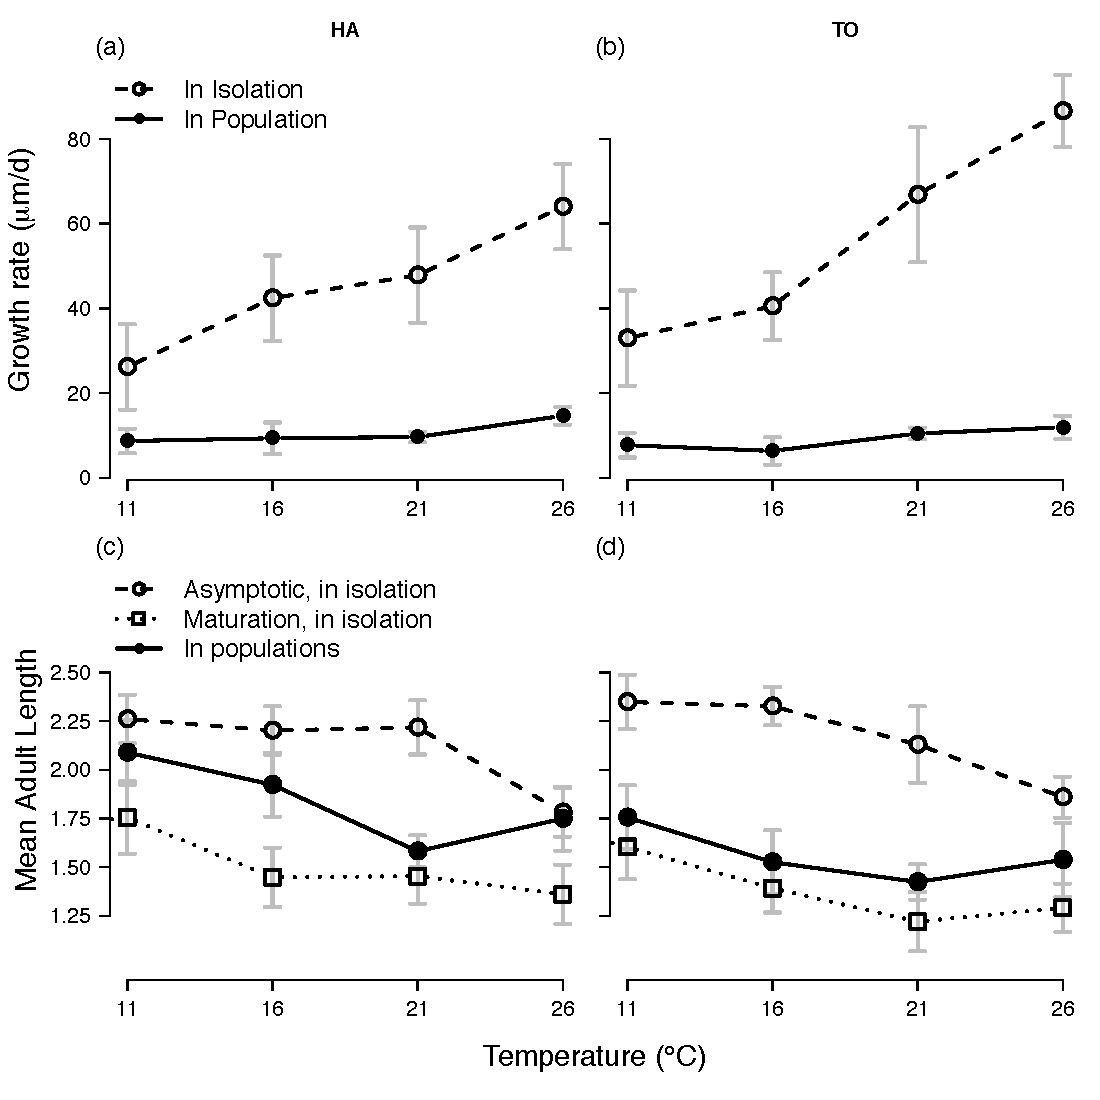
\includegraphics[width=0.95\textwidth]{5_ChapExp3/fig/Fig3} 
\caption[\lofimage{5_ChapExp3/fig/Fig3}Thermal reaction norms of the growth
rates]{ Thermal reaction norms of the growth rates (a, b, mean and 95\% confidence intervals) of the clones HA (a) and TO (b) measured on isolated individuals (dashed lines)
and on cohorts within populations (strait lines). Thermal reaction norms for
mean body length (c, d): mean body length at maturity (dotted lines) and
asymptotic length of isolated individuals (dashed lines) compared with mean
adult body length in populations (strait lines).}
\label{Fig5-3}
\end{figure}

\subsubsection{Maturation and asymptotic size}

Isolated individuals of both strains followed almost identical thermal reaction
norms for maturation and asymptotic sizes (Figure \ref{Fig5-3}c,d). First,
asymptotic size decreased with temperature (F$_{1,38}=73$, p$<0.0001$) without any
difference between the clonal lineages: the intercepts at 11$\degres$C (F$_{1,37}=2$,
p$=0.16$) and the slope of decrease with temperature increase
(F$_{1,37}=0.6$, p$=0.30$) were identical for TO and HA. Second, size at
maturity was stable between 11 to $\approx$21$\degres$C and decreased after 21$\degres$C
(Figure \ref{Fig5-3}c,d).
In contrast to isolated individuals, the effect of temperature on the mean adult length differed between the two clones:
in populations, TO individuals stopped growing shortly after reaching their size
at maturity: the asymptotic length in populations closely followed the reaction
norm for size at maturity (Figure \ref{Fig5-3}c,d). On the other hand, the HA individuals
reached a size intermediate between the maturation and maximum asymptotic sizes
in cold environments (11, 16$\degres$C) but at 21$\degres$C the adults where much smaller in
populations that when isolated. Remarkably, the main qualitative difference
between the reaction norms measured on isolated individuals and in populations
is that the mean adult length in populations increased between 21$\degres$C and 26$\degres$C for
both clonal lineages ( p$<0.0001$).

\subsection{Density dependence and temperature}

To further study what may have caused the reshaping of the thermal reaction
norms in the populations, we have studied, for both clonal lineages, how the
relative growth rates and GEBM respond to temperature and population density. We
used the adult density as the covariable of the population state since total
adult surface represents on average 90\% of the biosurface and we know from
other experiments that adults outcompete juveniles in resource acquisition and
therefore play a central role in the density dependence effects.

\subsubsection{Density dependence and relative growth rates}

For every temperature, the relative growth rate of cohorts of juveniles
decreased with adult density (p$<0.0001$ Figure \ref{Fig5-4}a,b, Table
\ref{tab5-2}). Juveniles from HA lineage grew on average faster than TO's
(F$_{1,4}=41$, p$<.0001$) but they suffered from a stronger negative effect of
density than TO ones (F$_{1,108}=20$, p$>.0001$).
For both lineages, increasing temperature reduces the cohorts’ relative growth
rates (F$_{1,46}=66$, p$<.0001$).

\subsubsection{Growth effort beyond maturation}

The response of GEBM to adult density and temperature differed quantitatively
but not qualitatively between the two lineages (Figure \ref{Fig5-4}c,d, Table
\ref{tab5-3}).
On average the growth effort of HA is higher than that of TO individuals
(F$_{1,39}=51.6$, p<.0001). For both lineages, the growth effort decreased with
increasing density (p<.0001): when adult density increased, the mean size reached by the cohorts
was closer to the size at maturity. The intensity of this density dependence
(slope of the decrease) in HA was about twice that of TO (Figure
\ref{Fig5-4}c,d, F$_{1,70}=28.1$, p<.0001) but within each lineage, it was not
affected by temperature (Table \ref{tab5-3}).

We also found that for the two lineages, the GEBM varies with temperature but
contrary to growth rate the effect of temperature was not linear.

\begin{figure}[!ht] % Figure 4 
\centering
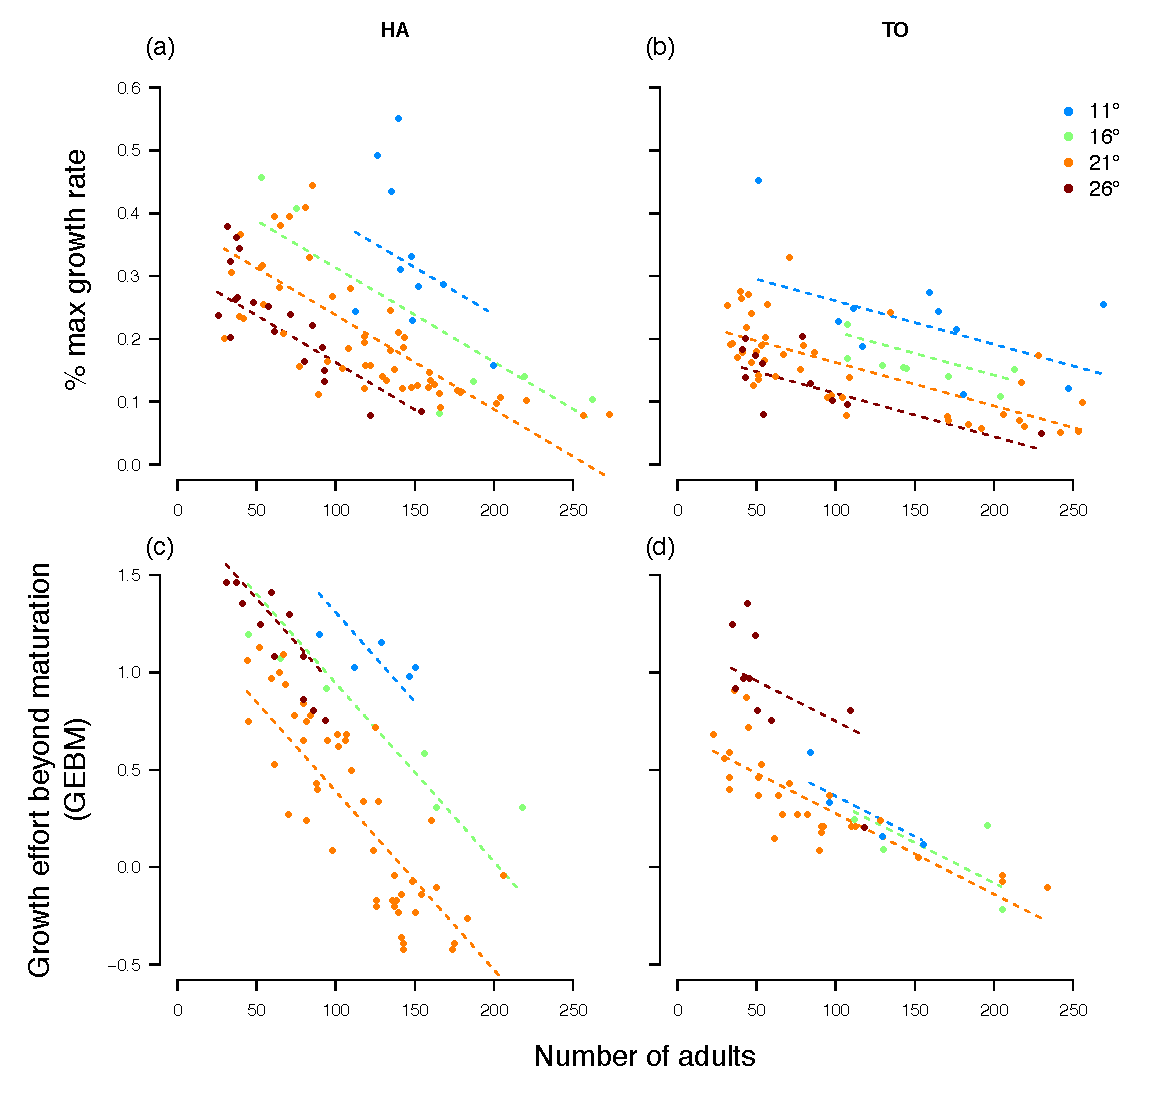
\includegraphics[width=0.95\textwidth]{5_ChapExp3/fig/Fig4} 
\caption[\lofimage{5_ChapExp3/fig/Fig4}Relative growth rates and adult
densities in populations]{ The relative growth rates (a, b, \% growth rate in
populations compared to the growth rates measured on isolated individuals) and adult densities measured in the populations raised under four different ambient temperatures for the clone
(a) HA and (b) TO lineages. (c, d) The growth effort beyond maturation -- a
measure of how much the individuals grow in the populations compared to their
body length when isolated -- and population density for the four temperatures.
The dotted lines are the predictions from the simplified models fitted on each
clone.
}
\label{Fig5-4}
\end{figure}

\subsubsection{Predicted thermal reaction norms}

In order to highlight how the \% growth rates and investment in growth (GEBM)
vary with temperature while controlling for density within clonal lineages, we
plotted the predicted \% growth and GEBM for a density of 100 adults (the
overall mean adult density observed in our populations, Figure \ref{Fig5-5}a,b) using the
models fitted to each lineage independently (Table \ref{tab5-2} and Table
\ref{tab5-3}). For both lineages, the \% growth rate decreased linearly with increasing temperature
(Figure \ref{Fig5-5}a) but the GEBM reaction norms have a U-shaped profile: GEBM decreased
linearly between 11° to 21 but increased at 26°C (Figure \ref{Fig5-5}b). The body length
increase observed at 26°C (Figure \ref{Fig5-5}) is remarkable since in most of the
populations maintained at 26°C, the mean adult body length was higher than the
asymptotic length of the isolated individuals at the same temperature (Figure
\ref{Fig5-4}c,d) while in some HA populations maintained at 21° some cohorts did
not even reach the length at maturity measured on isolated individuals (Figure
\ref{Fig5-4}c, negative values).

\begin{figure}[!ht] % Figure 5
\centering
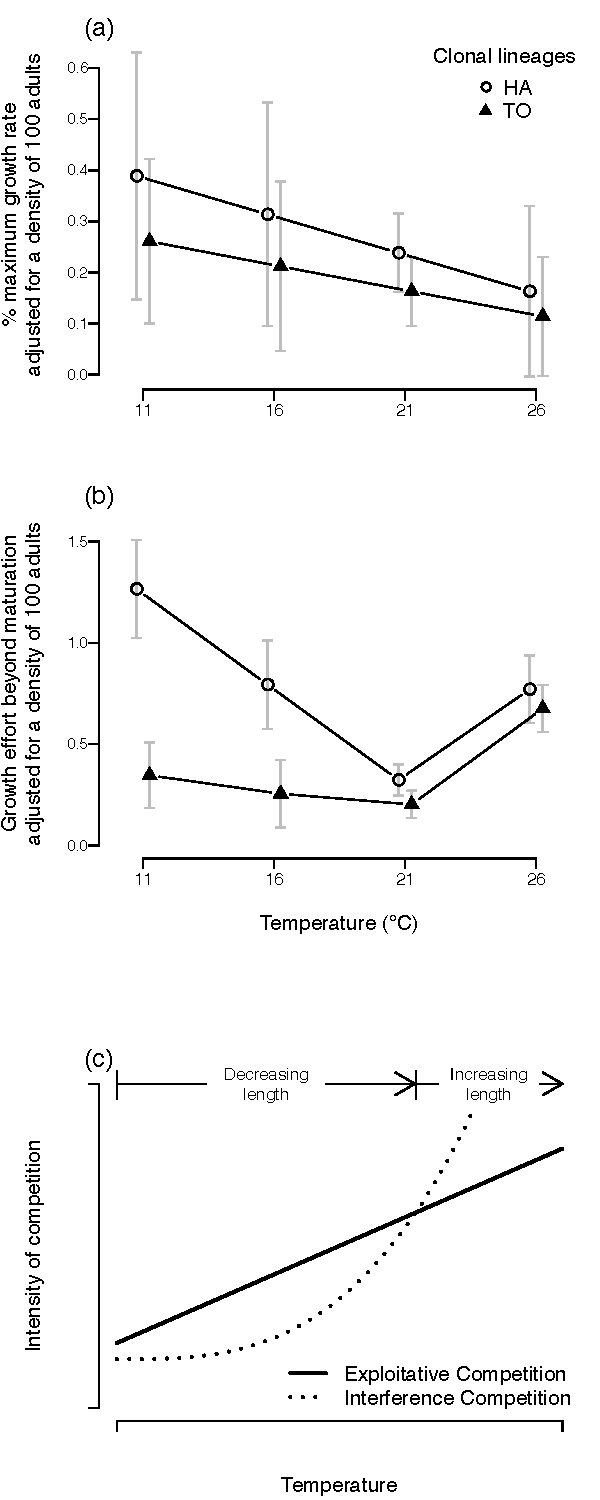
\includegraphics[height=0.8\textheight]{5_ChapExp3/fig/Fig5} 
\caption[\lofimage{5_ChapExp3/fig/Fig5}Thermal reaction norms of relative
growth rate and GEBM]{ The thermal reaction norms of relative growth rate (a)
and growth effort beyond maturation (b) for the two lineages. Predicted values from the fitted models
(mean ± 95\% confidence intervals) scaled for a density of 100 adults. (c)
Possible changes in the relative exploitative and interference competition in
the populations: as temperature increases, the intensity of interference
competition may prevail, thus favouring larger individuals.}
\label{Fig5-5}
\end{figure}

\section{Discussion}

We have combined and compared some measurements of life-history traits of
isolated individuals to measurements made in experimental populations.

\subsection{Thermal reaction norms of isolated individuals.}

The thermal reaction norms measured on isolated individuals revealed a positive
effect of temperature on growth rates and a negative effect on adult body
lengths. From 11°C to 26°C, the average growth rate is multiplied by three while
the adult length decreases by about 20\%. This proves that, as many other
ectotherms \autocites{atkinson1994a,angilletta2009a}, our
Collembola follow the temperature size rule: individuals raised under cold ambient temperature grow
more slowly but become larger when adults \autocites{angilletta2003a}.
While previous work has described similar effects of temperature on collembolan
juvenile growth rates
\autocites{birkemoe2000a,driessen2007a,ellers2008a,ellers2011a}, or on size at
maturity \autocites{stam1996a}, it is to our knowledge the first experimental
evidence of such plastic adjustment of adult body length to ambient temperature in collembolans.

The comparison of our two clones, known for their contrasted biodemographic
strategies \autocites{tully2006a}, revealed only little genetic
variation on the slope of these individual reaction norms. This result is similar to what has
been observed in another Collembola \autocites{driessen2007a}.

\subsection{Density dependence in the populations}

We report here the first description of experimental population dynamics under a
temperature gradient, with a close monitoring of size structure dynamics
(Figure \ref{Fig5-S2}). Our experimental populations have in general a
size-structure distribution with two distinct modes: they are mainly composed of
juveniles and adults (Figure \ref{Fig5-2}e,f). Periodically, a group of
juveniles manages to grow and join the adults (Figure \ref{Fig5-S2}).

The reaction norms measured in populations differed from those of isolated
individuals. Both growth rates and body lengths were on average reduced in the
populations (Figure \ref{Fig5-3}) probably because of the strong competition for
resources in the populations. In this experiment we provided a constant amount
of food in each rearing box and let the populations settle. Thus the populations
reached dynamical equilibrium states where the food limits the number, the mean
size and investment in reproduction of adults. These equilibria result from
complex feedback loops between genetically variable life history strategies
\autocites{tully2008a} and density dependence effects \autocites{kokko2007a} that
can have here two main origins: competition for food and space limitation. The
amount of food given every week was the same across the whole range of
temperature. The food pellets were eaten in one or two days on average and the
individuals were then fasting until the end of the week. Competition for food
was probably the main factor regulating population size which itself regulated
the cohort growth rates and adult lengths. These negative effects of density
were visible on two scales: (1) by comparing the traits measured in populations
to traits measured on isolated individuals (Figure \ref{Fig5-3}) and by
comparing populations with different adult densities (Figure \ref{Fig5-4}).
The effect of density is very strong here especially on the growth rates which reached only about 20 or 30\% of the
growth rates of isolated individuals (Figure \ref{Fig5-4}). This strong effect
of density wipes out, in the populations, most of the plastic adjustments of phenotypic
traits to temperature (Figure \ref{Fig5-4}): the temperature size rule is broken
down by density dependent effects.

The comparison of the two clones revealed some significant genetic variation in
the intensity of this density dependence: for both traits, HA suffered more than
TO from an increase of density and this was true over the whole range of
temperature. This genetic variation could arise from genetic differences in the
juvenile sensibility to adult density but also from genetic differences in the
level of competitive pressure the adults put on the juveniles in the
populations. To disentangle these two potential explanations one would need to
compare the juvenile growth rates and the size they reach as adults when placed
with adults of the two different clones.

\subsection{Thermal reaction norms in the populations}

Under our thermal gradient, we also found that the phenotypic plasticity
observed on isolated individuals vanished or even reversed in populations. The
growth rates of cohorts in populations was highly reduced by competitive
interactions and it remained almost constant across the temperature gradient
(Figure \ref{Fig5-3}a,b). Yet, by comparing these growth rates with those measured on
isolated individuals and by controlling for the densities of the populations, we
found that mean relative growth rates decreases with temperature: the negative
effect of density strengthen with increasing temperature (Figure \ref{Fig5-5}).
This result suggests that the intensity of competition for the resource in the population is
increasing with the temperature, an explanation that is consistent with the
higher biochemical and physiological rates at high
temperatures \autocites{gillooly2002a}.

The mean adult body length in the populations is negatively correlated with the
adult densities. Moreover, from 11°C to 21°C the growth effort beyond maturation
decreases: in warm environments, the mean adult length in populations gets
closer to length at maturation observed on isolated individuals. Again, this is
coherent with an increase of the intensity of competition with temperature. In
our experimental system, the food consumption rate increases with temperature
while the resource's renewal rate is kept constant. In such conditions, theory
predicts a magnified competitive advantage of small individuals when the
temperature rises \autocites{ohlberger2011a}. Bigger individuals
should normally be outcompeted by small ones in hot environments. In our experiments, this effect
is probably dominant over a large range of temperatures (11° to 21°) and could
explain the observed decrease of body length and growth effort beyond maturation
from 11 to 21° (Figure \ref{Fig5-3}c,d, Figure \ref{Fig5-5}b)

Yet, we observed an increase in the mean body length of adults in the
populations between 21° and 26° (Figure \ref{Fig5-3}) which could not be
explained by a lower density in the containers or by the direct effect of
temperature. This result suggests that the increase of the exploitative
competition does not explain all the density dependence effects in our
populations (Figures \ref{Fig5-3} and \ref{Fig5-5}). Direct interactions between
individuals (interference competition) can also have a role in the regulation of
a population's dynamics
\autocites{park1962a,schoener1983a,anholt1990a,smallegange2006a,nakayama2010a,mccormick2012a}.
Interference between individuals reduces the individuals’ feeding rates because
of the time spend to these behavioural interactions to the detriment of feeding
\autocites{smallegange2006a} and because of the
extra energetic cost associated to agonist interactions \autocites{briffa2007a}.
In case of a significant difference in size and strength between the interacting individuals,
the dominant denies the smaller individuals access to resource with a minimal
effort. Therefore the cost of interference for the dominating individual is
negligible whereas it is maximum for the smaller ones, counteracting the effect
of exploitative competition. Juvenile and adult collembolans have the same
ecology and they share the same food resources and it is very likely that
interference competition occurs between small and large individuals in our
populations at the benefit of the later.

While increasing exploitative competition favours smaller individuals,
increasing interference competition can have the opposite effect. The relative
importance of both types of competition could shape the plastic adjustment of
adult body length in populations. If interference competition increases faster
than exploitative competition with temperature, its effect could prevail beyond
a certain temperature and thus favour bigger individuals (Figure \ref{Fig5-5}c).
We believe that as temperature accelerates individual life cycles of our ectotherms, a
progressive mismatch between the frequency of food supply - once a week at every
temperature - and the frequency with which the springtails are in demand of food
- twice in a full reproductive cycle - leads to an increase in this interference
competition. A greater proportion of the population may be ready to compete for
the food pellet when dropped in the box at hotter temperatures. The U-shape
reaction norm observed in populations could be explained by an increase of both
type of competition with temperature: the first one - exploitative competition -
induces a decrease of body length up to 21° whereas the second one - an
interaction competition to access food that relates to interference competition
- induces an increase of body length at higher temperatures (Figure \ref{Fig5-5}c).

\section{Conclusion}

We managed by independent measurements of life history traits on isolated
individuals, or in populations, to show how the density dependence is itself
affected by temperature. This highlights a need to disentangle the different
components of density dependence to predict how populations will react to the
overall modification of temperature such as that induced by the anthropogenic
climate change. Changes in resource availability may have a major impact. In
particular, changes not only in the mean quantity of resources but also on their
temporal availability may greatly affect size distribution in populations.

\section{Theoretical perspectives}

Physiologically structured population models \autocites{metz1986a,de-roos1992a} constitute a framework that is increasingly used to study
population dynamics \autocites{marty2011a,moenickes2011a}.
By explicitly modelling the body length, as well as the rates of living at an individual
level, one is able to encompass a broader range of possible dynamics. Being
individually based, this also provides a theoretical framework to add to
individual competitive interactions along with exploitative competition to study
their roles in driving the dynamics of a structured population. Calibrating such
a model at different temperatures would allow one to investigate how the
temperature affects the level of exploitative and interference competition in
the population, and interact with both forms of competition in driving the
population's dynamics.

















\newpage
\section{Supplementary material}

\begin{figure}[!ht] % Figure S1 
\centering
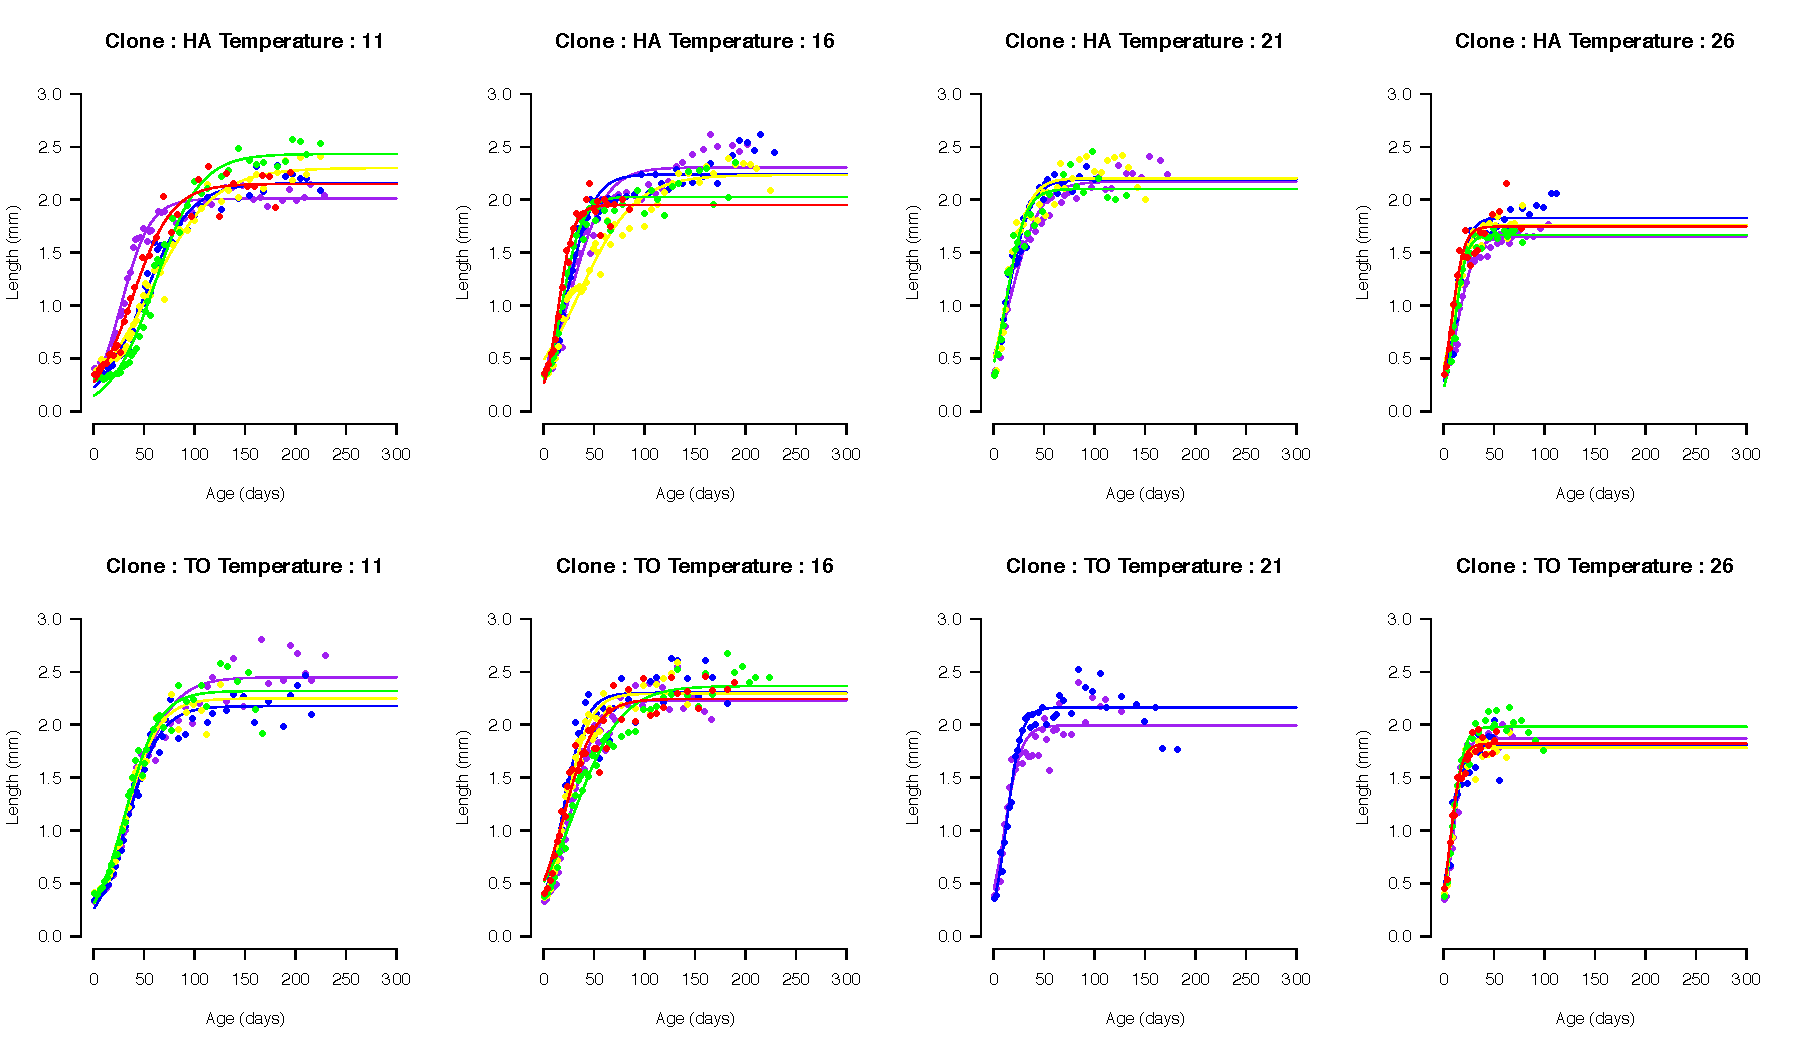
\includegraphics[width=0.95\textwidth]{5_ChapExp3/fig/FigS1}
\caption[\lofimage{5_ChapExp3/fig/FigS1}Individual growth trajectories]{
The 33 individual growth trajectories used to estimate the reaction norms for mean growth rates, size at maturity and adult asymptotic body lengths}
\label{Fig5-S1}
\end{figure}

\newpage

\begin{figure}
  \centering 
  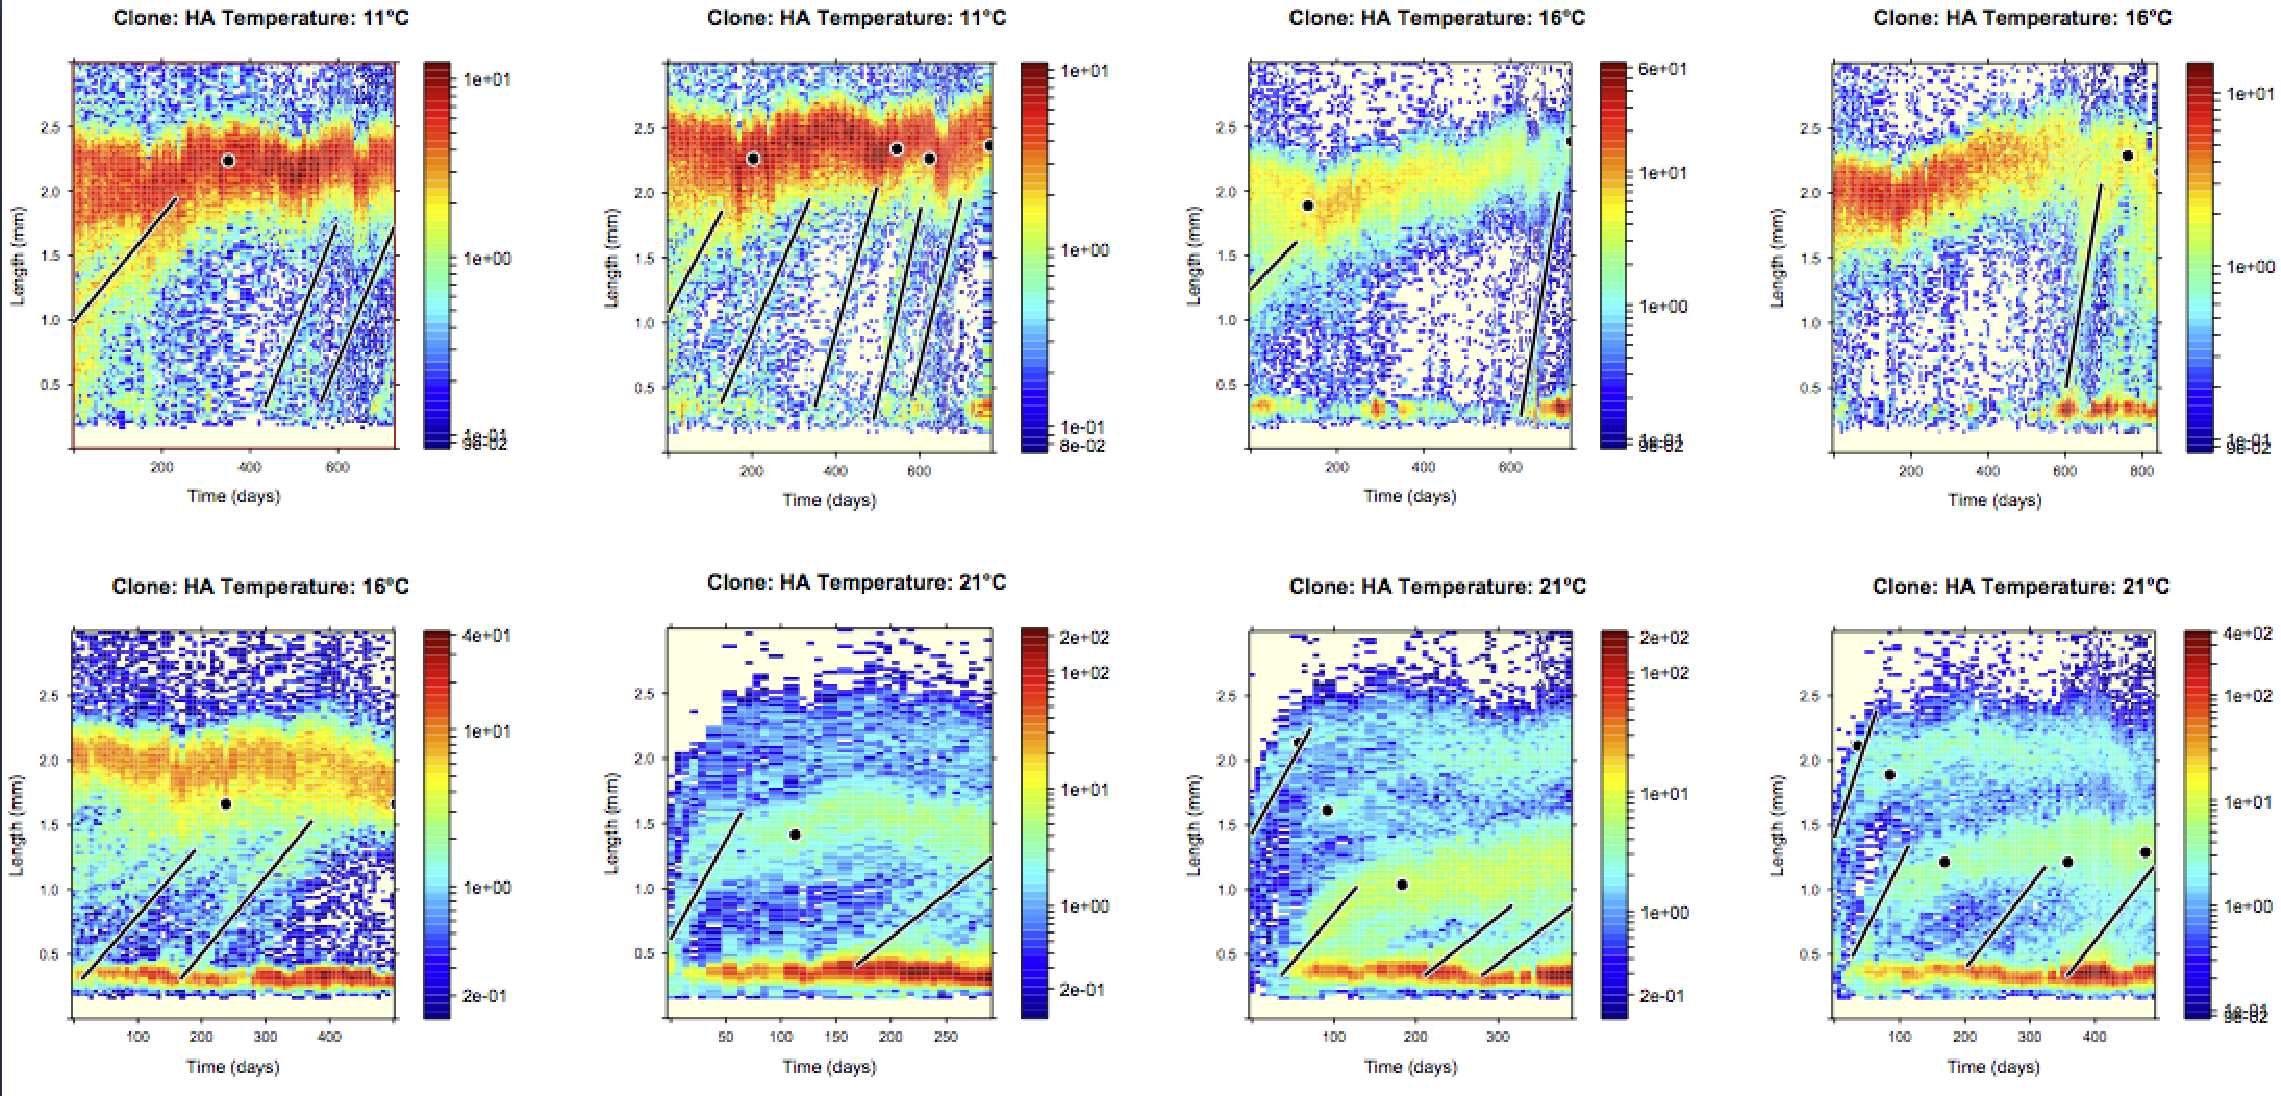
\includegraphics[width=0.85\textwidth]{5_ChapExp3/fig/FigS2-1} 
  %\caption{Here are the first two figures of a continued figure.}
  \phantomcaption
 % \label{Fig5-S2}
\end{figure}
\begin{figure}
  \centering 
  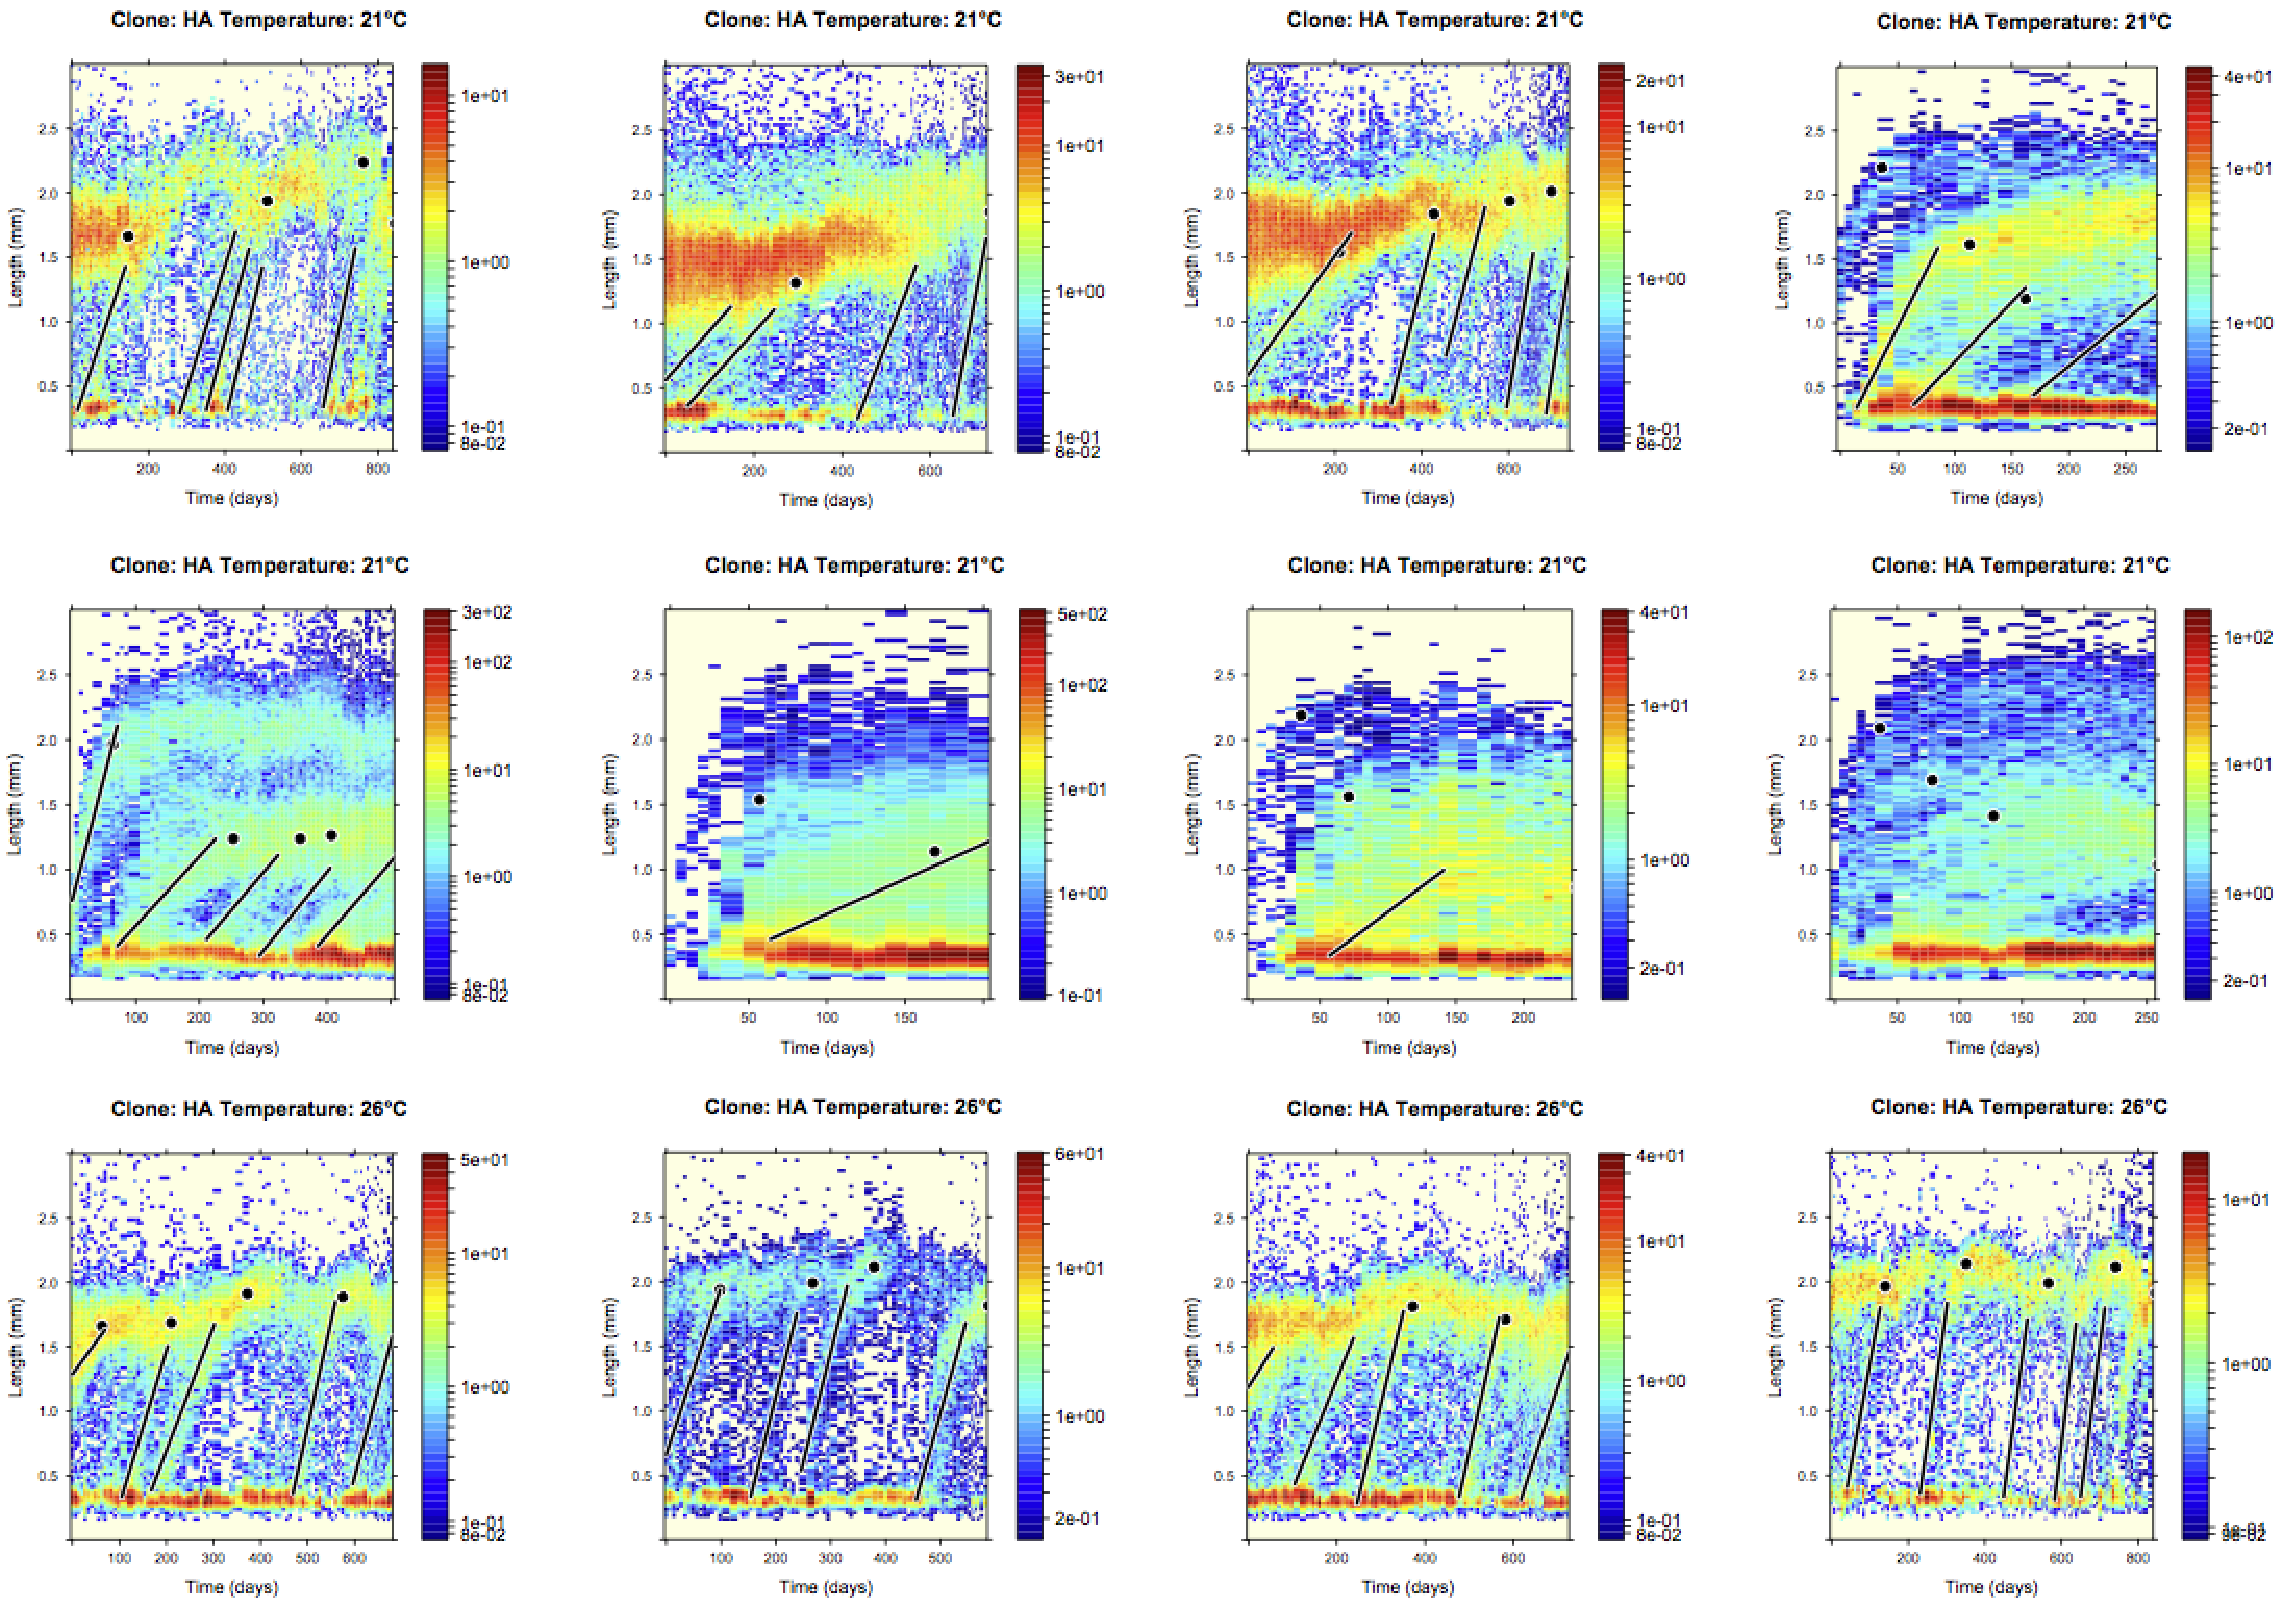
\includegraphics[width=0.85\textwidth]{5_ChapExp3/fig/FigS2-2} 
  \caption[\lofimage{5_ChapExp3/fig/FigS2-4}The
  structure time diagrams of the 46 populations used in our analysis]{The
  structure time diagrams of the 46 populations used in our analysis (clones TO and HA maintained at 11, 16, 21 and 26$\degres$C). The points underlines the
  measurements of adult body lengths of recently recruited cohorts. The black
  lines show the measures of cohort growth rates in the populations.}
  %\phantomcaption
  %\label{Fig5-S2}
\end{figure}
\begin{figure}
  \centering 
  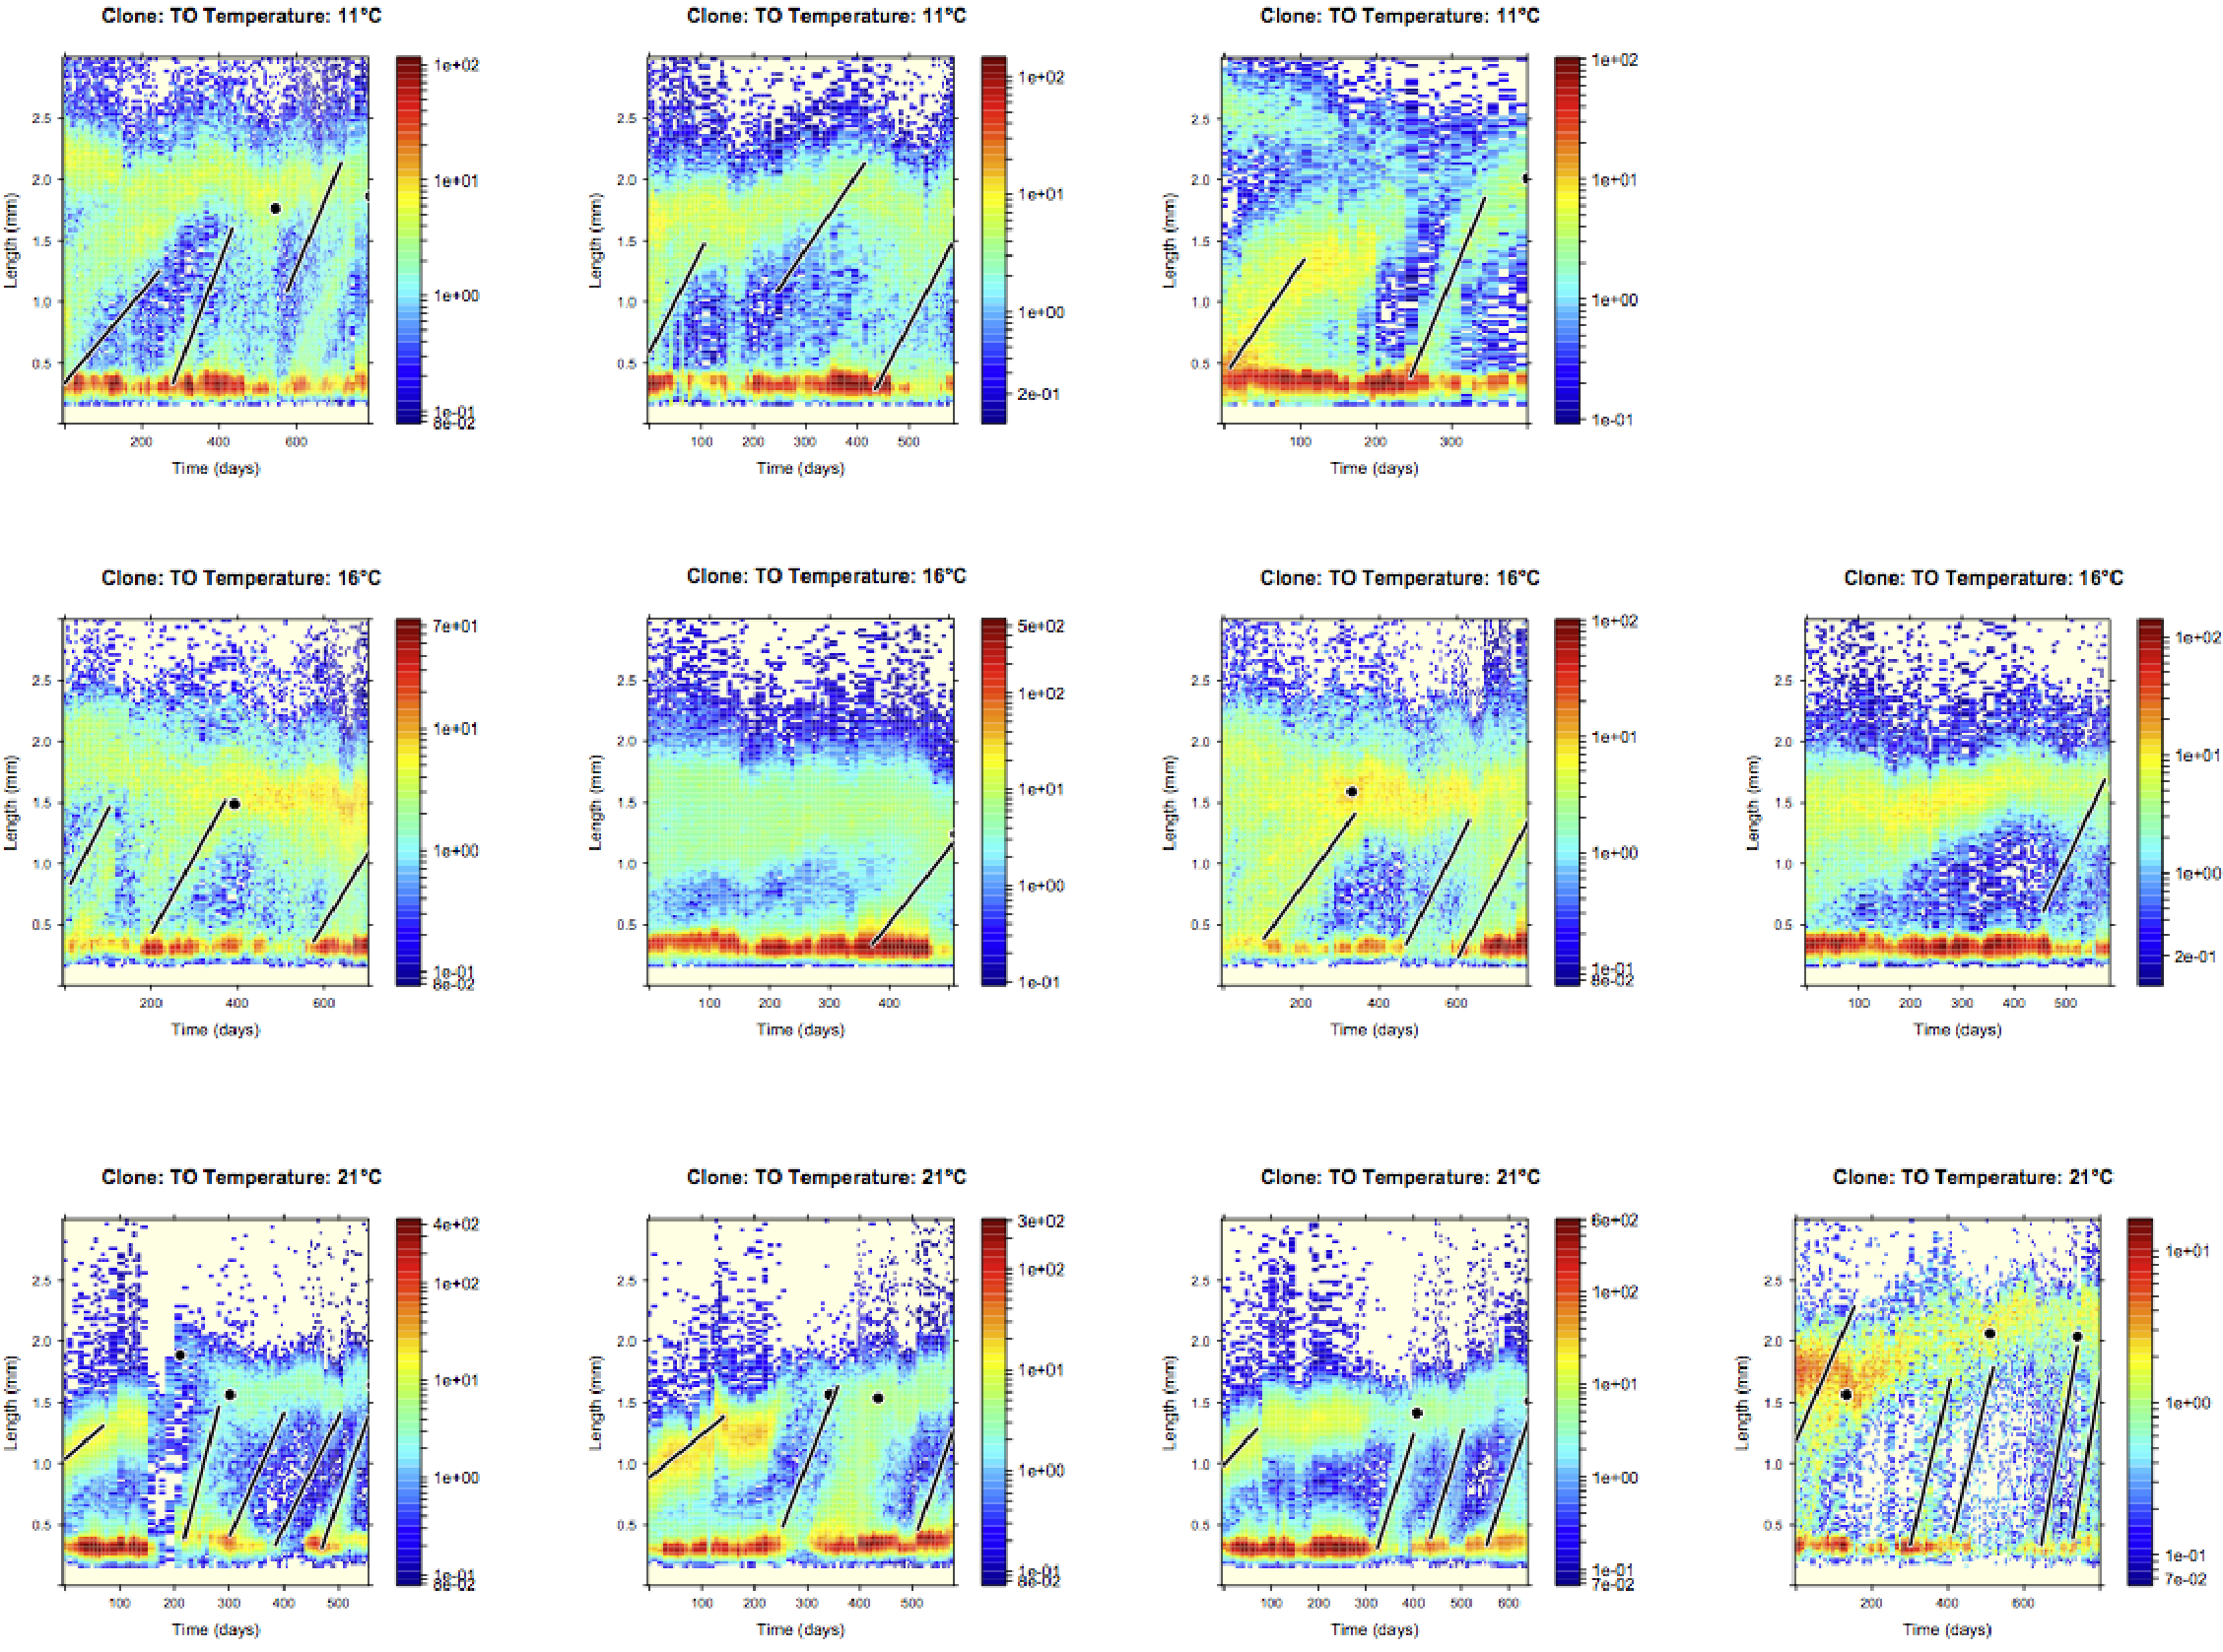
\includegraphics[width=0.85\textwidth]{5_ChapExp3/fig/FigS2-3} 
  %\caption{Here are the first two figures of a continued figure.}
  \phantomcaption
 % \label{Fig5-S2}
\end{figure}
\begin{figure}
  \ContinuedFloat 
  \centering 
  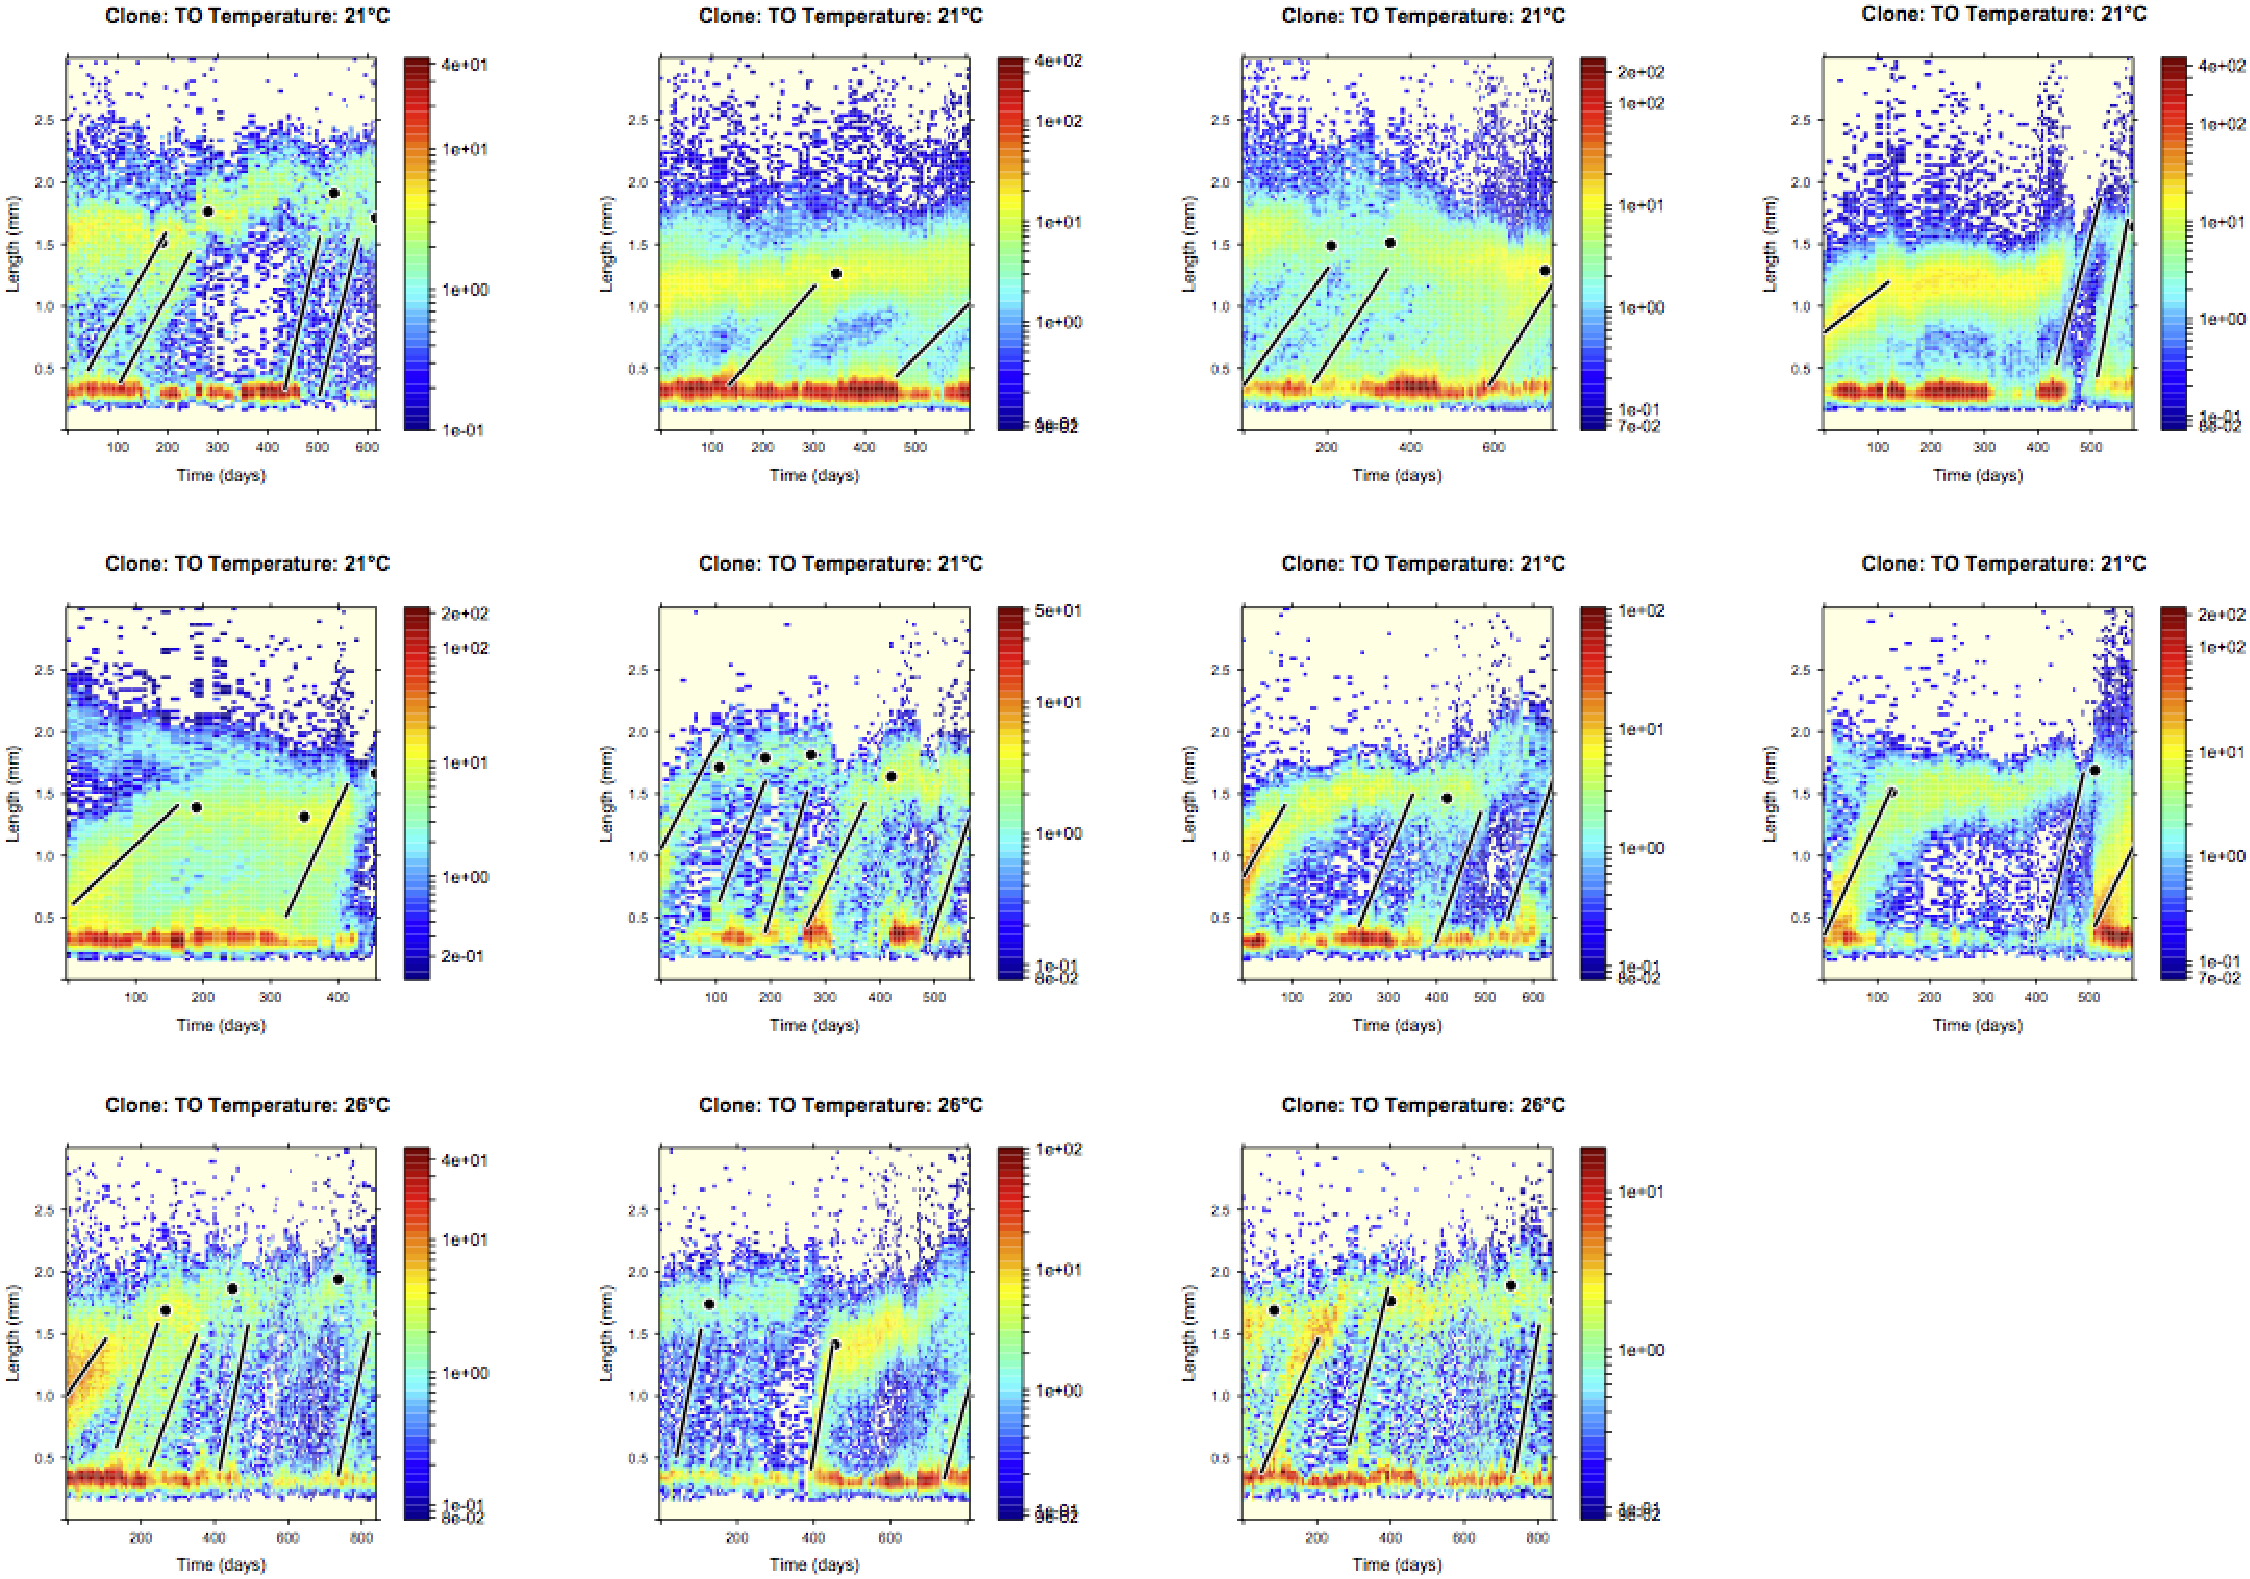
\includegraphics[width=0.85\textwidth]{5_ChapExp3/fig/FigS2-4}
  \caption[]{
  The structure time diagrams of the 46 populations used in our analysis (clones
  TO and HA maintained at 11, 16, 21 and 26$\degres$C). The points underlines the
  measurements of adult body lengths of recently recruited cohorts. The black
  lines show the measures of cohort growth rates in the populations.}
  \label{Fig5-S2}
\end{figure}